\documentclass[usenames,dvipsnames,tikz]{standalone}
\usepackage{xcolor}
\colorlet{tBlue}{RoyalBlue!35!Cerulean}
\colorlet{tRed}{Red}
\definecolor{tGreen}{HTML}{569909}
\definecolor{tOrange}{HTML}{FA7602}
\usepackage{tikz}
\usepackage{standalone}
\begin{document}
	
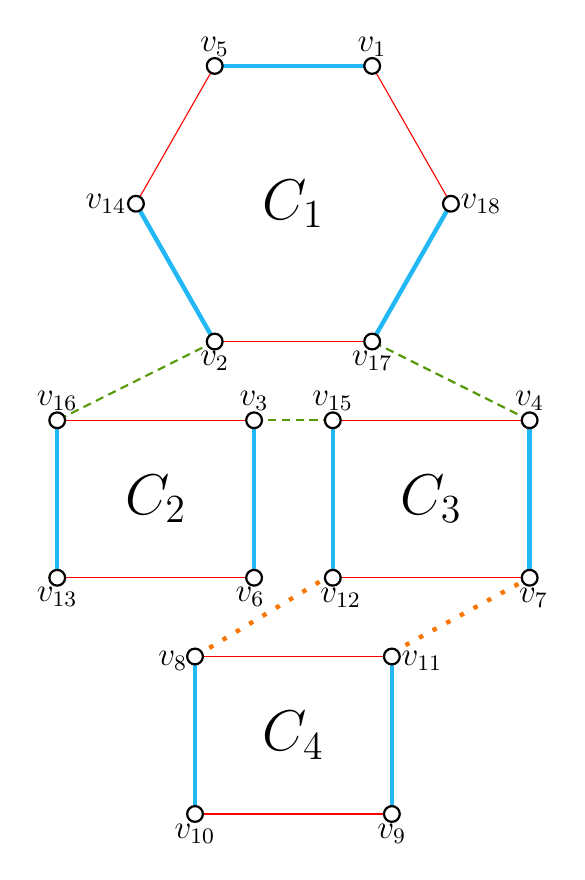
\begin{tikzpicture}
%v1=1, v2=1, v3=2, v4=2, v5=3, v6=4, v7=4, v8=5, v9=5, v10=6, v11=6, v12=6, v13=6, v14=7, v15=8, v16=9
%\draw [help lines] (-1,-1) grid (8, 13);

%C1 - blue
\draw [ultra thick, tBlue] (2.5,9.5) -- (4.5,9.5); 
\draw [ultra thick, tBlue] (2.5,6) -- (1.5,7.75); 
\draw [ultra thick, tBlue] (4.5,6) -- (5.5,7.75); 

%C2 - blue
\draw [ultra thick, tBlue] (0.5,3) -- (0.5,5); 
\draw [ultra thick, tBlue] (3,3) -- (3,5); 

%C3 - blue
\draw [ultra thick, tBlue] (4,3) -- (4,5); 
\draw [ultra thick, tBlue] (6.5,3) -- (6.5,5); 

%C4 - blue
\draw [ultra thick, tBlue] (2.25,0) -- (2.25,2); 
\draw [ultra thick, tBlue] (4.75,0) -- (4.75,2);

%C1 - red
\draw [tRed] (2.5,6) -- (4.5,6); 
\draw [tRed] (1.5,7.75) -- (2.5,9.5); 
\draw [tRed] (5.5,7.75) -- (4.5,9.5); 

%C2 - red
\draw [tRed] (0.5,3) -- (3,3); 
\draw [tRed] (0.5,5) -- (3,5); 

%C3 - red
\draw [tRed] (4,3) -- (6.5,3); 
\draw [tRed] (4,5) -- (6.5,5);

%C4 - red
\draw [tRed] (2.25,0) -- (4.75,0); 
\draw [tRed] (2.25,2) -- (4.75,2); 
%----------------------------
%Bridges
\draw [thick, densely dashed, tGreen] (2.5,6) -- (0.5,5); 
\draw [thick, densely dashed, tGreen] (3,5) -- (4,5); 
\draw [thick, densely dashed, tGreen] (6.5,5) -- (4.5,6); 

\draw [ultra thick, loosely dotted, tOrange] (4,3.05) -- (2.25,2); 
\draw [ultra thick, loosely dotted, tOrange] (4.75,2.05) -- (6.5,3); 
%----------------------------


%C1 - vertices
\draw [fill=white, thick] (2.5,6) circle [radius = 0.1]; %v2
\draw [fill=white, thick] (4.5,6) circle [radius = 0.1]; %v17
\draw [fill=white, thick] (1.5,7.75) circle [radius = 0.1]; %v14
\draw [fill=white, thick] (5.5,7.75) circle [radius = 0.1]; %v18
\draw [fill=white, thick] (2.5,9.5) circle [radius = 0.1]; %v5
\draw [fill=white, thick] (4.5,9.5) circle [radius = 0.1]; %v1

%C2 - vertices
\draw [fill=white, thick] (0.5,3) circle [radius = 0.1]; %v13
\draw [fill=white, thick] (3,3) circle [radius = 0.1]; %v6
\draw [fill=white, thick] (0.5,5) circle [radius = 0.1]; %v16
\draw [fill=white, thick] (3,5) circle [radius = 0.1]; %v3

%C3 - vertices
\draw [fill=white, thick] (4,3) circle [radius = 0.1]; %v12
\draw [fill=white, thick] (6.5,3) circle [radius = 0.1]; %v7
\draw [fill=white, thick] (4,5) circle [radius = 0.1]; %v15
\draw [fill=white, thick] (6.5,5) circle [radius = 0.1]; %v4

%C4 - vertices
\draw [fill=white, thick] (2.25,0) circle [radius = 0.1]; %v10
\draw [fill=white, thick] (4.75,0) circle [radius = 0.1]; %v5
\draw [fill=white, thick] (2.25,2) circle [radius = 0.1]; %v8
\draw [fill=white, thick] (4.75,2) circle [radius = 0.1]; %v11

%C1 - labels
\node [below] at (2.5,6) {\large{$v_2$}};
\node [below] at (4.5,6) {\large{$v_{17}$}};
\node [left] at (1.5,7.75) {\large{$v_{14}$}};
\node [right] at (5.5,7.75) {\large{$v_{18}$}};
\node [above] at (2.5,9.5) {\large{$v_5$}};
\node [above] at (4.5,9.5) {\large{$v_1$}};

%C2 - labels
\node [below] at (0.5,3) {\large{$v_{13}$}};
\node [below] at (2.95,3) {\large{$v_6$}};
\node [above] at (0.5,5) {\large{$v_{16}$}};
\node [above] at (3,5) {\large{$v_3$}};

%C3 - labels
\node [below] at (4.1,2.99) {\large{$v_{12}$}};
\node [below] at (6.55,2.99) {\large{$v_7$}};
\node [above] at (4,5) {\large{$v_{15}$}};
\node [above] at (6.5,5) {\large{$v_4$}};

%C4 - labels
\node [below] at (2.25,0) {\large{$v_{10}$}};
\node [below] at (4.75,0) {\large{$v_9$}};
\node [left] at (2.275,1.95) {\large{$v_8$}};
\node [right] at (4.75,1.95) {\large{$v_{11}$}};

%Component labels
\node at (3.5,7.75) {\huge{$C_1$}};
\node at (1.75,4) {\huge{$C_2$}};
\node at (5.25,4) {\huge{$C_3$}};
\node at (3.5,1) {\huge{$C_4$}};


\end{tikzpicture}
	
\end{document}
